Рассмотрим описаные алгоритмы умножения матриц умножения матриц $ А[MxN] $ и $ B[NxQ] $ с результирующей матрицей умножения матриц $ C[MxQ] $.

\section{Стандартный алгоритм умножения}
Данный алгоритм непосредственно использует вышеприведённую формулу. Для вычисления каждого элемента матрицы С совершается циклический обход k элементов из таблиц А и B.

Схема алгоритма приведена на рисунке 2.1
\begin{figure}[h]
	\begin{center}
		{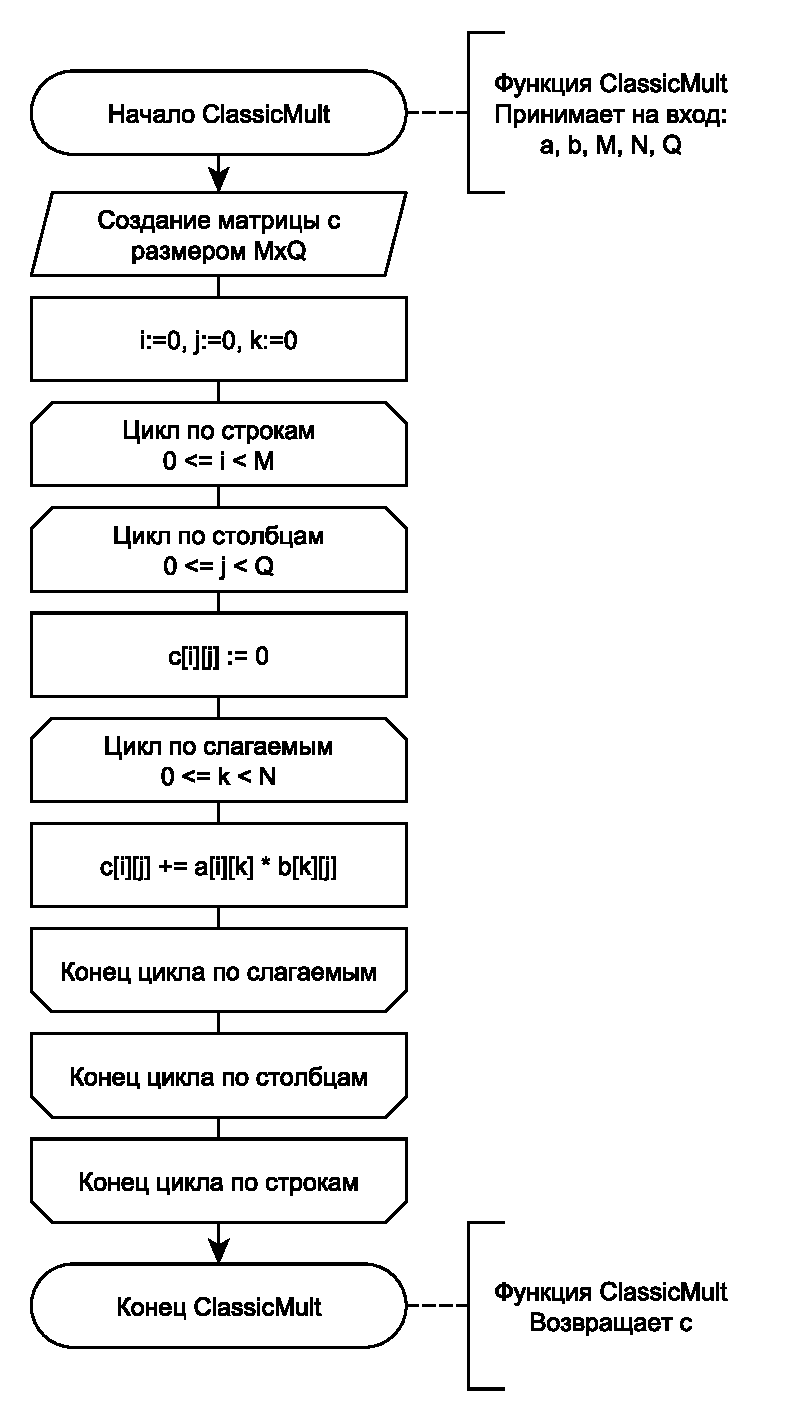
\includegraphics[height=20cm, width = 14cm]{Classic}}
		\caption{Стандартный алгоритм умножения}
	\end{center}
\end{figure}


\section{Алгоритм умножения параллельный по строкам}
Как было отмечено выше, вычисление каждого элемента матрицы является независимым. Поэтому возможна следующая параллельная версия данного алгоритма. Пусть производится работа с $T$ потоками. В таком случае, i-й поток будет производить вычисление строк $i$, $i+T$, $i+2T$, ..., $((M-i) mod T)*T + i$.

Схема алгоритма приведена на рисунках 2.2, 2.3
\begin{figure}[h]
	\begin{center}
		{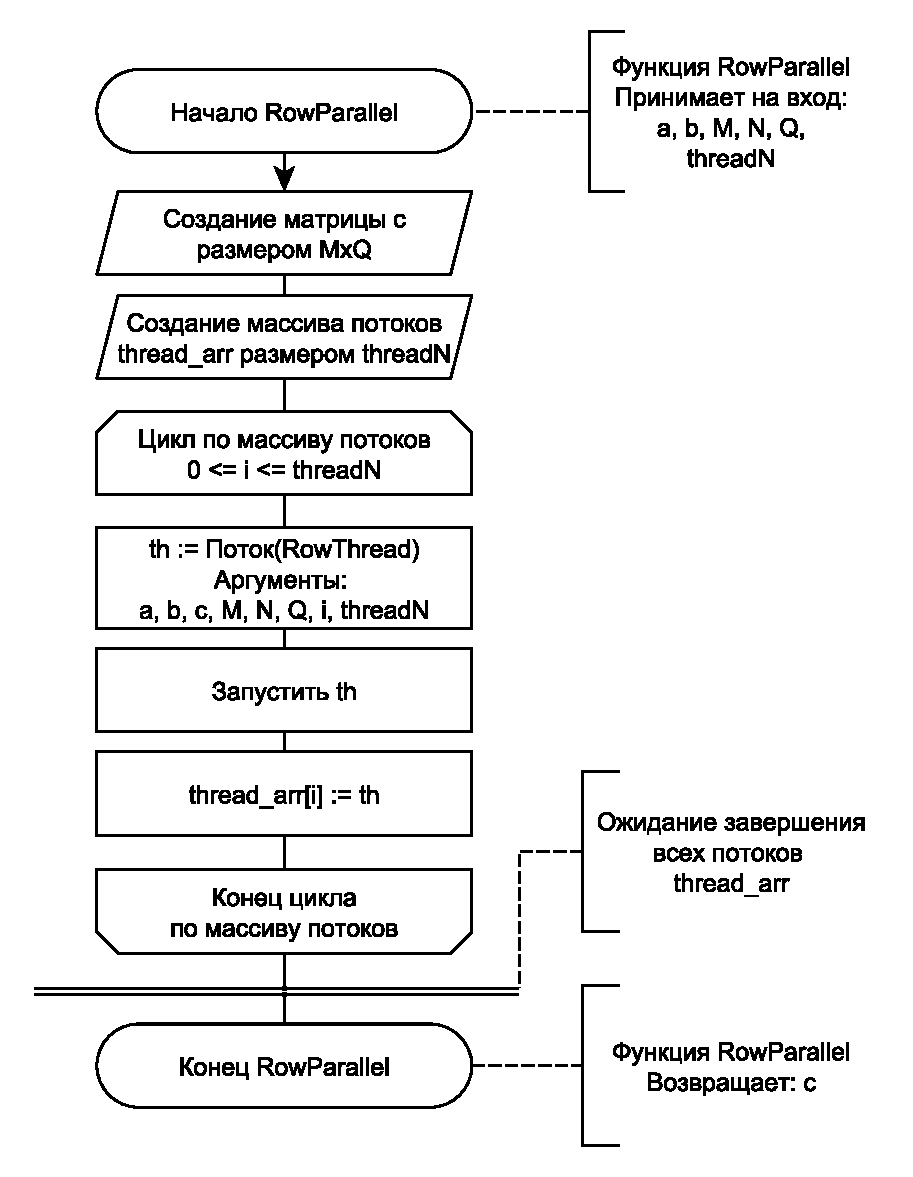
\includegraphics[height=17cm, width = 17cm]{MainRow}}
		\caption{Алгоритм умножения параллельный по строкам (главный поток)}
	\end{center}
\end{figure}
\begin{figure}[h]
	\begin{center}
		{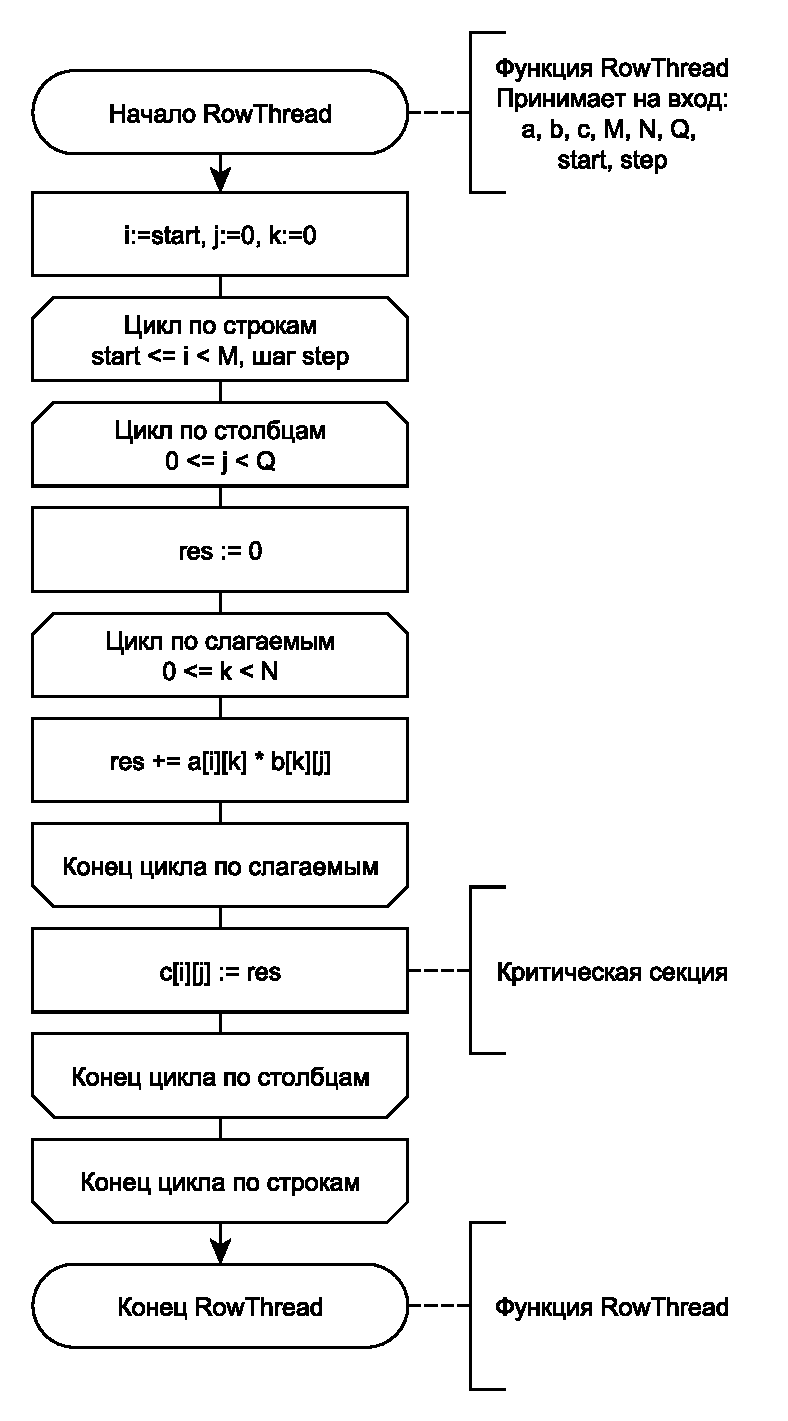
\includegraphics[height=20cm, width = 15cm]{WorkRow}}
		\caption{Алгоритм умножения параллельный по строкам (рабочий поток)}
	\end{center}
\end{figure}


\section{Алгоритм умножения параллельный по столбцам}
В силу независимости вычислений каждого элемента, аналогично можно организовать и параллельное вычисление значений в столбцах матрицы $C$. В таком случае, i-й поток будет производить вычисление столбцов $i$, $i+T$, $i+2T$, ..., $((Q-i) mod T)*T + i$.

Схема алгоритма приведена на рисунках 2.4, 2.5
\begin{figure}[h]
	\begin{center}
		{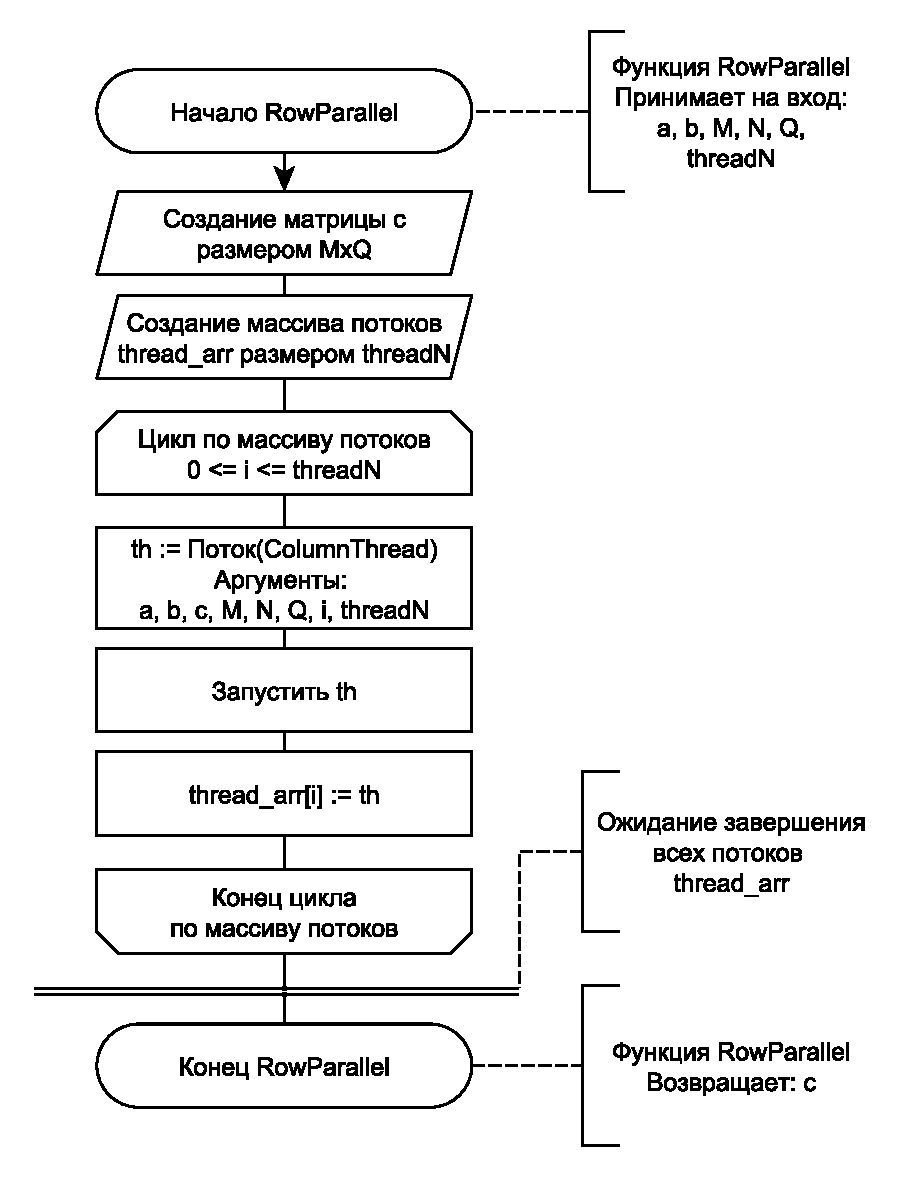
\includegraphics[height=17cm, width = 17cm]{MainColumn}}
		\caption{Алгоритм умножения параллельный по столбцам (главный поток)}
	\end{center}
\end{figure}
\begin{figure}[h]
	\begin{center}
		{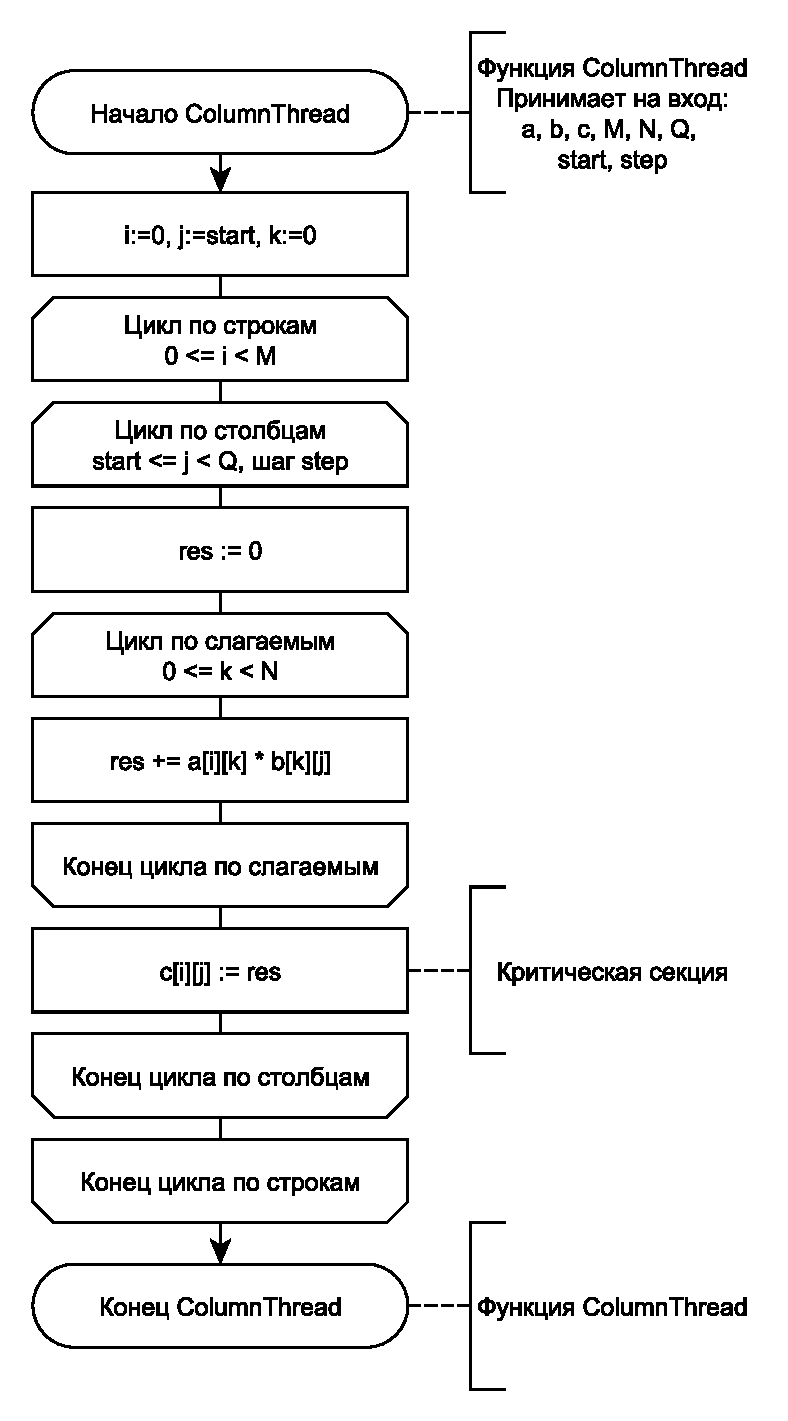
\includegraphics[height=20cm, width = 15cm]{WorkColumn}}
		\caption{Алгоритм умножения параллельный по столбцам (рабочий поток)}
	\end{center}
\end{figure}

\section{Требования к программному обеспечению}
Для полноценной проверки и оценки алгоритмов необходимо выполнить следующее.
\begin{enumerate}
	\item Предоставить выбор алгоритма для умножения, обеспечить возможность консольного ввода двух матриц и количества используемых потоков (в случае выбора многопоточного алгоритма). Программа должна вывести результирующую матрцу.
	\item Реализовать функцию замера процессорного времени, затраченного функциями.
\end{enumerate}


\section{Заготовки тестов}
При проверке алгоритма необходимо будет использовать следующие классы тестов:
\begin{itemize}
	\item один поток, несколько потоков;
	\item матрицы размером 1x1;
	\item пустые матрицы;
\end{itemize}

\section*{Вывод}
Результатом конструторской части стало схематическое описание алгоритмов умножения матриц, сформулированны тесты и требования к программному обеспечению.



